\section{Neurobiology}\label{sec:neurobiology}
\qquad \todo{straightforward recap of the basics, more focus on topic-relevant details}



\subsection{Units for propofol concentration}
Some papers~\cite{iwakiri_individual_2005} cite propofol concentrations in $\SI{}{\frac{\micro\gram}{\milli\litre}}$,
while others~\cite{kitamura_effects_2003, mcdougall_propofol_2008} use $\SI{}{\micro\molar}$ (micromolar =
$\SI{}{\frac{\micro\mol}{\litre}}$).
To get comparable numbers, we first need to establish the following relation for Propofol (molar mass: $\SI{178
.27}{\gram}$):
\[ \SI{1}{\frac{\micro\gram\hspace{0.5em}\text{\tiny{Propofol}}}{\milli\litre}}  =
\frac{ \SI{1}{\frac{\micro\gram}{\milli\litre}}}{\SI{178.27}{\frac{\gram}{\mol}}} = \SI{5.609}{\micro\molar} \]
In this work, we will settle on $\SI{}{\micro\molar}$
and only mention values in $\SI{}{\frac{\micro\gram}{\milli\litre}}$ where they are taken from a source,
but then provide the converted value as well.


\subsection{Realistic propofol concentrations during general anaesthesia (GA)}\label{subsec:realistic-prop-conc-during-ga}

During GA, effect-site concentrations ($c_{e}$, concentration near the synaptic receptors) of propofol may easily range
up to
$\SI{5}{\frac{\micro\gram}{\milli\litre}} (\approx\SI{28}{\micro\molar})$.
Loss of Consciousness (LOC) occurs on average at $c_e \sim\SI{2.0}{\frac{\micro\gram}{\milli\litre}} (\approx\SI{11
.2}{\micro\molar})$,
while the Return of Consciousness (ROC) averages at $c_e \sim\SI{1.8}{\frac{\micro\gram}{\milli\litre}}
(\approx\SI{10.1}{\micro\molar})$.
Both values may vary substantially for individual subjects.
LOC has a strong tendency to occur at higher concentrations than ROC~\cite{iwakiri_individual_2005,
    ferreira_patterns_2020}.
Throughout GA, effect-site concentration is commonly derived from measured
blood-plasma concentration ($c_p$) using more or less complex Pharmacokinetic (PK)-Models
(e.g.\ ~\cite{eleveld_general_2014, liang_pharmacokinetics-neural_2015}),
as direct measurement is impractical for obvious reasons.
Since our model will work with $c_{e}$ directly, we will disregard this for now - however, it should be kept in mind.


\subsection{Effects of propofol on the IPSP}

Research on the effect of propofol on the IPSC (Inhibitory Post-Synaptic Current) and EPSC
has shown that propofol strongly affects the IPSP decay time \cite{kitamura_effects_2003, mcdougall_propofol_2008}.
The EPSP and the amplitude of the IPSP are unaffected by propofol.
Effect-site concentrations at clinically relevant levels increase the IPSP decay time
significantly (e.g.\ around $\SI{10}{\micro\molar}$ the decay time roughly doubles)~\cite{kitamura_effects_2003}.

Using the data-points from~\cite{kitamura_effects_2003}
and assuming a very rough manual logarithmic fit (see Fig.~\ref{fig:lambda_fit}),
the function
        \[ \mathscr{D}(c_{e}) = 0.65*ln((c_{e}/2)+1)+1 \]
will be used to calculate the decay-time factor $\lambda$ from a given
effect-site concentration in $\SI{}{\micro\molar}$.

As there unfortunately were only a few data-points (and none above $\SI{10}{\micro\molar}$,
leaving a large part of the relevant parameter space empty),
a computational model-fit might have over-valued those points.
A visually fitted logarithmic function (assuming eventual effect saturation) seemed like a sensible choice
for this use-case.
However, since inter-subject variations are substantial in any case,
the exact values do not matter as much as the order of magnitude.


\begin{figure}[H]
    \centering
    \pgfplotsset{compat = newest}
    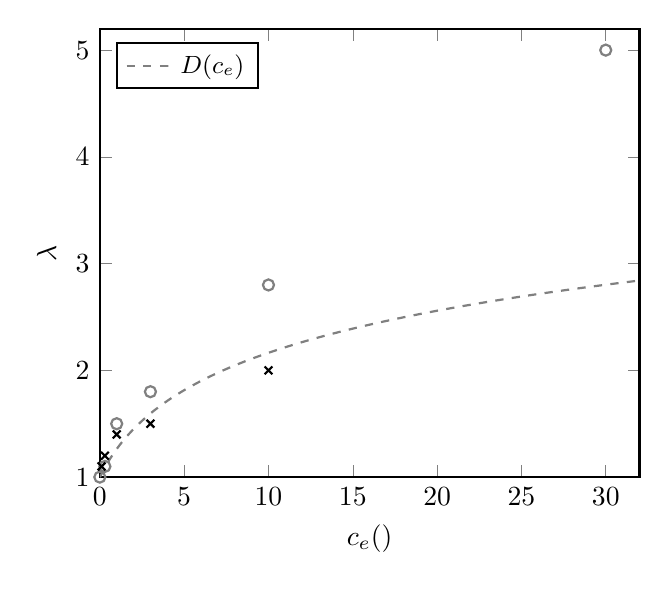
\begin{tikzpicture}
        \begin{axis}
            [
            xmin = 0, xmax = 32,
            ymin = 1, ymax = 5.2,
            xlabel = {$c_{e} (\SI{}{\micro\molar})$},
            ylabel = {$\lambda$},
            legend pos=north west,
            domain = 0:32,
            samples = 50,
            smooth,
            thick,
            scatter/classes={a={mark=o,draw=gray}, b={mark=x,draw=black}}
            ],
            %\addplot[dashed, gray]{3.8*ln((x/18)+1)+1};
            %\addplot[gray       ]{0.5*ln((x)+1)+1};
            \addplot[dashed,gray]{0.65*ln((x/2)+1)+1};
            \legend{\small$\mathscr{D}(c_{e})$};
            %\addplot[green]{0.9*ln((x/4)+1)+1};
            %\addplot[red]{1.15*ln((x/4)+1)+1};
            \addplot[scatter,only marks,scatter src=explicit symbolic] table[meta=label] {
                x y label
                0 1 a
                0.3 1.1 a
                1 1.5 a
                3 1.8 a
                10 2.8 a
                30 5.0 a
                0.1 1.1 b
                0.3 1.2 b
                1 1.4 b
                3 1.5 b
                10 2 b
                };

                %\draw [gray, dotted] (axis cs:0,2.5) -- (axis cs:18.1,2.5)-- (axis cs:18.1,0);
        \end{axis}
    \end{tikzpicture}

    \caption{very rough manual logarithmic fit of decay-time factor to measured values
    from~\cite{kitamura_effects_2003}.}
    \label{fig:lambda_fit}
\end{figure}

\subsection{Hysteresis of propofol}
If the state of a system depends not only on its parameters, but also the systems history,
this dependency is called hysteresis.
The human body often reacts differently to the same concentration of a drug,
depending on whether the concentration is rising or decaying.
Hysteresis is well documented during propofol-induced GA~\cite{kuizenga_quantitative_1998,
    iwakiri_individual_2005,
    sepulveda_evidence_2018,ferreira_patterns_2020, su_hysteresis_2020}.
The most prominent effect being a counter-clockwise hysteresis for LOC and ROC (as mentioned
in~\ref{subsec:realistic-prop-conc-during-ga}).
The effects on responsiveness of subjects usually start at higher concentrations than they end.
While some of that effect might be caused by inaccurate PK-Models,
misgauging the actual effect-site concentration,
there is a growing body of research that supports the notion that the observed effect is independent of
pharmacokinetic interference~\cite{hutt_progress_2011, su_hysteresis_2020}.
% Therories of reasons: - re-initiation more complex than shutdown, phase-transitions

\begin{figure}[H]
    \centering
    \pgfplotsset{compat = newest}
    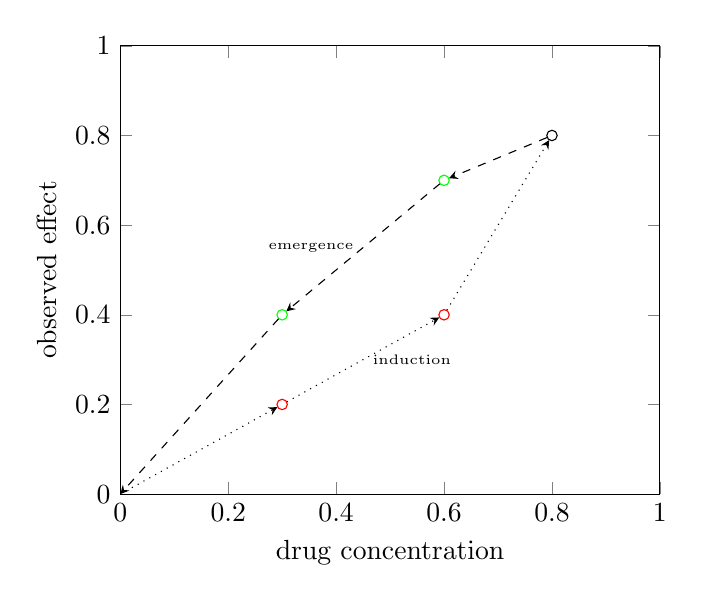
\begin{tikzpicture}
        \begin{axis}
            [
            xmin = 0, xmax = 1,
            ymin = 0, ymax = 1,
            xlabel = {drug concentration},
            ylabel = {observed effect},
            ],
            \node[circle, scale=0.4, draw=red] (I1) at (axis cs:0.3,0.2) {};
            \node[circle, scale=0.4, draw=red] (I2) at (axis cs:0.6,0.4) {};
            \node[circle, scale=0.4, draw=black] (I3) at (axis cs:0.8,0.8) {};

            \node[circle, scale=0.4, draw=green] (E1) at (axis cs:0.6,0.7) {};
            \node[circle, scale=0.4, draw=green] (E2) at (axis cs:0.3,0.4) {};

            \draw [ dotted, -stealth] (axis cs:0,0) -- (I1) ;
            \draw [ dotted, -stealth] (I1) -- (I2)
            node[midway, right,font=\tiny]{induction};
            \draw [dotted, -stealth] (I2) -- (I3);

            \draw [dashed, -stealth] (I3) -- (E1) ;
            \draw [dashed, -stealth] (E1) -- (E2)
            node[midway, left, font=\tiny]{emergence};
            \draw [dashed, -stealth] (E2) -- (axis cs:0.0,0.0);
        \end{axis}
    \end{tikzpicture}

    \caption{Example of counter-clockwise drug hysteresis}
    \label{fig:hystersis_in_general}
\end{figure}
